\documentclass[a4paper,10pt]{article}

\usepackage{Raf_Packages}

\graphicspath{{./sources/images/}}

%variables
%\renewcommand	{\partie}		{Résistance Des Matériaux}
\renewcommand	{\titre}		{Liaison pivot}


\renewcommand{\dx}[1]  {\ensuremath{{\color{red}\text{d}x_{#1}}}}
\renewcommand{\dy}[1]  {\ensuremath{{\color{red}\text{d}y_{#1}}}}
\renewcommand{\dtheta}[1]  {\ensuremath{{\color{red}\text{d}\theta_{#1}}}}


\begin{document}
	
	\begin{center}
        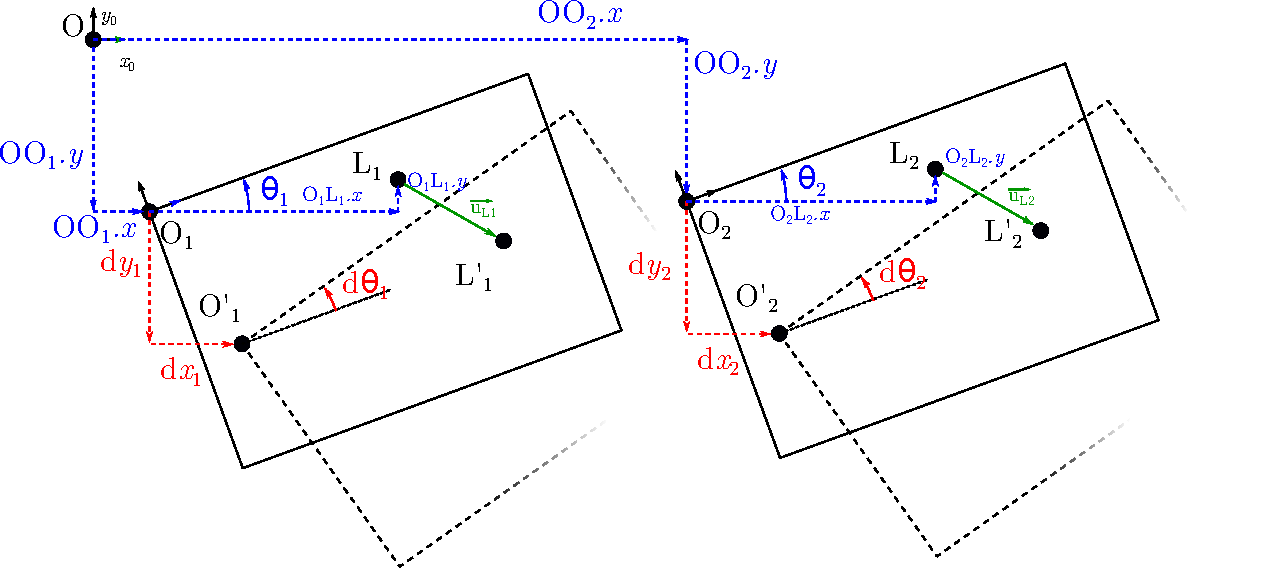
\includegraphics[width=\linewidth]{pivot.pdf}
	\end{center}

	
	
	\subsection{Force de $L_2$ sur $L_1$}
	% ------------------------------------------------
	
        \begin{align*}
            \resAM{L_2}{L_1}    =&  k\vecteur{L_1'L_2'}   \\
                    =&  k\left(\vecteur{L_1'L_1}+\vecteur{L_1L_2}+\vecteur{L_2L_2'}\right)\\
                    =&  k\left(-\vDep{L_1}{1}{0}+\vecteur{L_1L_2}+\vDep{L_2}{2}{0}\right)\\
                    =&  k\left(-\left(\vDep{O_1}{1}{0}+\vecteur{L_1O_1}\wedge\vPetiteRot10\right)
                                +\vecteur{L_1L_2}
                                +\left(\vDep{O_2}{2}{0}+\vecteur{L_2O_2}\wedge\vPetiteRot20\right)
                                \right)\\
                    =&  k\left(-
                            \vColonne{\dx1\\\dy1\\0}{\bB0} + \vColonne{O_1L_1.x\\O_1L_1.y\\0}{\bB0}\wedge\vColonne{0\\0\\\dtheta1}{\bB0}\right.\\
                    &       +\vecteur{L_1L_2}\\
                    &       +\left.\vColonne{\dx2\\\dy2\\0}{\bB0} - \vColonne{O_2L_2.x\\O_2L_2.y\\0}{\bB0}\wedge\vColonne{0\\0\\\dtheta2}{\bB0}\right)\\
                    =&  k\left(-
                            \vColonne{\dx1\\\dy1\\0}{\bB0} + \vColonne{\dtheta1O_1L_1.y\\-\dtheta1O_1L_1.x\\0}{\bB0}\right.\\
                    &       +\vecteur{L_1L_2}\\
                    &       +\left.\vColonne{\dx2\\\dy2\\0}{\bB0} - \vColonne{\dtheta2O_2L_2.y\\-\dtheta2O_2L_2.x\\0}{\bB0}\right)\\
%                     =&  k\left(-
%                             \vColonne{\dx1\\\dy1\\0}{\bB0} + \vColonne{\dtheta1(O_1L_1.y\cos(\theta_1)+O_1L_1.x\sin(\theta_1))\\\dtheta1(O_1L_1.y\sin(\theta_1)-O_1L_1.x\cos(\theta_1))\\0}{\bB0}\right.\\
%                     &       +\vecteur{L_1L_2}\\
%                     &       +\left.\vColonne{\dx2\\\dy2\\0}{\bB0} - \vColonne{\dtheta2(O_2L_2.y\cos(\theta_2)+O_2L_2.x\sin(\theta_2))\\\dtheta2(O_2L_2.y\sin(\theta_2)-O_2L_2.x\cos(\theta_2))\\0}{\bB0}\right)
            =&      k\vColonne{
                            -\dx1 + \dtheta1 \left(O_1L_1.y\right)
                            +\dx2 - \dtheta2 \left(O_2L_2.y\right)
                            +L_1L_2.x
                            \\
                            -\dy1 - \dtheta1 \left(O_1L_1.x\right)
                            +\dy2 + \dtheta2 \left(O_2L_2.x\right)
                            +L_1L_2.y
            }{\bB0}
        \end{align*}
        
        
    \subsection{Moment}
    %-------------------------
    
        \begin{align*}
            \momAM{O_1'}{2}{1}   =&  \vecteur{O_1'L_1'}\wedge\resAM{2}{1}  \\
                                =&  \left(\vecteur{O_1'O_1}+\vecteur{O_1L_1}+\vecteur{L_1L_1'}\right)
                                \wedge\resAM{2}{1}  \\
                                =&  \left(-\vDep{O_1}{1}{0}+\vecteur{O_1L_1}+\vDep{L_1}{1}{0}\right)\wedge\resAM{2}{1}  \\
                                =&  \left(\cancel{-\vDep{O_1}{1}{0}}+\vecteur{O_1L_1}+\left(\cancel{\vDep{O_1}{1}{0}}+\vecteur{L_1O_1}\wedge\vPetiteRot10\right)\right)\wedge\resAM{2}{1}  \\
                                =&  \left(
                                    \vColonne{O_1L_1.x\\O_1L_1.y\\0}{\bB0}-\vColonne{O_1L_1.x\\O_1L_1.y\\0}{\bB0}\wedge\vColonne{0\\0\\\dtheta1}{\bB0}
                                \right)\wedge\resAM{2}{1}  \\
                                =&  k
                                    \vColonne{O_1L_1.x-\dtheta1O_1L_1.y\\O_1L_1.y+\dtheta1O_1L_1.x}{\bB0}
                                \wedge
                                \vColonne{
                                    -\dx1 + \dtheta1 \left(O_1L_1.y\right)
                                    +\dx2 - \dtheta2 \left(O_2L_2.y\right)
                                    +L_1L_2.x
                                    \\
                                    -\dy1 - \dtheta1 \left(O_1L_1.x\right)
                                    +\dy2 + \dtheta2 \left(O_2L_2.x\right)
                                    +L_1L_2.y
                            }{\bB0}\\
                           \momAM{O_1'}{2}{1}\cdot\vz{} =&k \times[\\
                            &O_1L_1.x
                                    \left(-\dy1 - \dtheta1 \left(O_1L_1.x\right)
                                    +\dy2 + \dtheta2 \left(O_2L_2.x\right)
                                    +L_1L_2.y\right)-\dtheta1O_1L_1.yL_1L_2.y
                                \\
                                 &   -\left(
                                        O_1L_1.y\left(-\dx1 + \dtheta1 \left(O_1L_1.y\right)
                                    +\dx2 - \dtheta2 \left(O_2L_2.y\right)
                                    +L_1L_2.x\right)+\dtheta1O_1L_1.xL_1L_2.x
                                    \right)]\\
                            =&k\times[\\
                            &\dx1\left(O_1L_1.y\right)
                            -\dy1\left(O_1L_1.x\right)
                            +\dtheta1\left(-O_1L_1.x^2-O_1L_1.y\ L_1L_2.y-O_1L_1.y^2+O_1L_1.x\ L_1L_2.x\right)\\
                            &-\dx2\left(O_1L_1.y\right)
                            +\dy2\left(O_1L_1.x\right)
                            +\dtheta2\left(O_1L_1.x\ O_2L_2.x+O_1L_1.y\ O_2L_2.y\right)\\
                            &+O_1L_1.x\ L_1L_2.y-O_1L_1.y\ L_1L_2.x]
        \end{align*}

        
    \subsection{Système}
    %-----------------------------
    
    
        Dans le système \[K\cdot U=F\], on a :
        \begin{align*}
            K &= \left[
                    \begin{array}{cccc}
                        -k  &   0   &   (kO_1L_1.y)   &   \dots
                        \\
                        0   &   -k  &   -(kO_1L_1.x)  &   \dots
                        \\
                        (k\ O_1L_1.y)    &   -(k\ O_1L_1.x)    &   k(O_1L_1.x\ L_1L_2.x-(O_1L_1.x^2+O_1L_1.y^2+O_1L_1.y\ L_1L_2.y))
                        & \dots
                    \end{array}
                \right.
                \\
           & \left.
                    \begin{array}{cccc}
                        \dots   &   k   &   0   &   -(kO_2L_2.y)
                        \\
                        \dots   &   0   &   k   &   (kO_2L_2.x)
                        \\
                        \dots
                        & -(k\ O_1L_1.y) & (k\ O_1L_1.x) & k(O_1L_1.x\ O_2L_2.x+O_1L_1.y\ O_2L_2.y)
                    \end{array}
                \right]
        \end{align*}
        
        \begin{align*}
            U = \vColonne{\dx1\\\dy1\\\dtheta1\\\dx2\\\dy2\\\dtheta2}{}
        \end{align*}
        
        \begin{align*}
            F   =   \vColonne{-kL_1L_2.x
                            \\-kL_1L_2.y
                            \\k\left(O_1L_1.y\ L_1L_2.x-O_1L_1.x\ L_1L_2.y\right)}{}
        \end{align*}




\end{document}
